\documentclass[tikz,border=5pt]{standalone}
\usepackage{amsmath}
\usepackage[T1]{fontenc}
\usetikzlibrary{calc}
\definecolor{region}{RGB}{96,115,182}
\definecolor{bounda}{RGB}{26,77,145}
\definecolor{boundb}{RGB}{181,70,65}
\definecolor{boundc}{RGB}{42,130,106}
\begin{document}

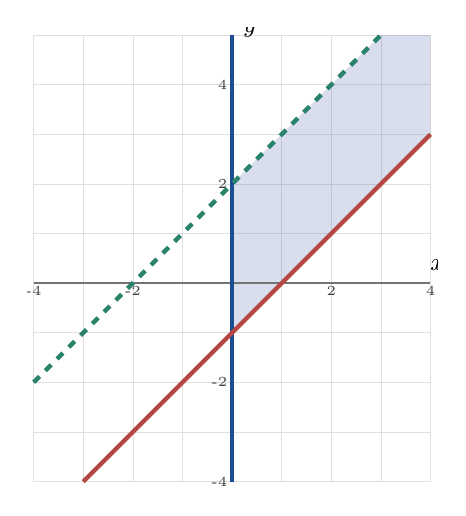
\begin{tikzpicture}
\begin{scope}[scale=0.63]
\clip (-4.12,-4.12) rectangle (4.15,5.15);
\draw[step=1,gray!25,very thin] (-4,-4) grid (4,5);
\fill[region,opacity=.24] (4,5) -- (3,5) -- (0,2) -- (0,-1) -- (4,3) -- cycle;
\draw[black!55,line width=.65pt] (0,-4) -- (0,5);
\draw[black!55,line width=.65pt] (-4,0) -- (4,0);
\draw[bounda,line width=1.55pt,solid] (0,-4) -- (0,5);
\draw[boundb,line width=1.55pt,solid] (4,3) -- (-3,-4);
\draw[boundc,line width=1.55pt,dashed] (-4,-2) -- (3,5);
\node[font=\tiny,anchor=north,inner sep=1pt,text=black!75] at (-4,0) {-4};
\node[font=\tiny,anchor=north,inner sep=1pt,text=black!75] at (-2,0) {-2};
\node[font=\tiny,anchor=north,inner sep=1pt,text=black!75] at (2,0) {2};
\node[font=\tiny,anchor=north,inner sep=1pt,text=black!75] at (4,0) {4};
\node[font=\tiny,anchor=east,inner sep=1.5pt,text=black!75] at (0,-4) {-4};
\node[font=\tiny,anchor=east,inner sep=1.5pt,text=black!75] at (0,-2) {-2};
\node[font=\tiny,anchor=east,inner sep=1.5pt,text=black!75] at (0,2) {2};
\node[font=\tiny,anchor=east,inner sep=1.5pt,text=black!75] at (0,4) {4};
\node[font=\small,anchor=west] at (3.8,.36) {$x$};
\node[font=\small,anchor=south] at (.36,4.75) {$y$};
\end{scope}
\end{tikzpicture}
\end{document}
